\documentclass[12pt]{article}
\usepackage{bbm}
\usepackage{fancyhdr}
\usepackage{titling}
\usepackage{enumitem}
\usepackage{amsmath}
\usepackage{dsfont}
\usepackage{amsfonts}
\usepackage{amssymb}
\usepackage{amsthm}
\usepackage{geometry}
\usepackage{tikz}
\usepackage{algorithm}
\usepackage{algpseudocode}
\geometry{verbose,tmargin=1in,bmargin=1in,lmargin=1in,rmargin=1in}
\renewcommand{\vec}[1]{\mathbf{#1}}
\newcommand{\dec}{\text{dec}}
\newcommand{\divi}{\mathbin{\textnormal{div}}}
\title{Homework 1}
\author{Satvik Prasad}
\date{}
\newtheorem{lemma}{Lemma}[section]
\fancypagestyle{plain}{%
  \fancyhf{}
  \fancyhead[L]{\theauthor}
  \fancyhead[R]{\thedate}
}
\pagestyle{plain}
\makeatletter
\def\@maketitle{%
  \newpage
  \null
  \vskip 1em%
  \begin{center}%
    \let \footnote \thanks
    {\LARGE \@title \par}%
    \vskip 1em%
  \end{center}%
  \par
\vskip 1em}
\makeatother
\usepackage{cmbright}

\newcommand{\mat}[1]{\mathbf{#1}}

% ---------- Probability theory ----------
% Core operators (optional argument-free; use as \E{X}, \Var{X}, \Cov{X}{Y})
\DeclareMathOperator{\EOp}{\mathbb{E}}
\DeclareMathOperator{\VarOp}{Var}
\DeclareMathOperator{\CovOp}{Cov}
\DeclareMathOperator{\CorrOp}{Corr}

\renewcommand{\P}[1]{\mathbb{P}\left(#1\right)}        % \P{A}
\newcommand{\E}[1]{\EOp\left[#1\right]}                % \E{X}
\newcommand{\Var}[1]{\VarOp\left(#1\right)}            % \Var{X}
\newcommand{\Cov}[2]{\CovOp\left(#1,\,#2\right)}       % \Cov{X}{Y}
\newcommand{\Corr}[2]{\CorrOp\left(#1,\,#2\right)}     % \Corr{X}{Y}
\newcommand{\SD}[1]{\operatorname{SD}\left(#1\right)}  % \SD{X}

% Subscripted versions, e.g. \Esub{\theta}{X}, \Psub{\theta}{A}
\newcommand{\Esub}[2]{\EOp_{#1}\left[#2\right]}
\newcommand{\Psub}[2]{\mathbb{P}_{#1}\left(#2\right)}

% Conditioning, indicators, independence
\newcommand{\given}{\,\middle|\,}                      % \E{X \given Y}
\newcommand{\ind}[1]{\mathbbm{1}\left\{#1\right\}}     % \ind{X > 0}
\newcommand{\indep}{\perp\!\!\!\perp}                  % X \indep Y
\newcommand{\iid}{\overset{\text{iid}}{\sim}}          % X_i \iid \Normal(0,1)

% Convergence
\newcommand{\convp}{\xrightarrow{\;p\;}}               % in probability
\newcommand{\convd}{\xrightarrow{\;d\;}}               % in distribution
\newcommand{\convas}{\xrightarrow{\text{a.s.}}}        % almost surely
\newcommand{\convLp}[1]{\xrightarrow{L^{#1}}}          % in L^p

% Probability spaces
\newcommand{\F}{\mathcal{F}}                           % sigma-algebra
\newcommand{\B}{\mathcal{B}}                           % Borel sigma-algebra
\newcommand{\pspace}{(\Omega, \F, \mathbb{P})}

% Common distributions
\newcommand{\Normal}{\mathcal{N}}
\newcommand{\Bern}{\operatorname{Bernoulli}}
\newcommand{\Bin}{\operatorname{Binomial}}
\newcommand{\Pois}{\operatorname{Poisson}}
\newcommand{\Unif}{\operatorname{Uniform}}
\newcommand{\Exp}{\operatorname{Exp}}
\newcommand{\Geom}{\operatorname{Geometric}}
\newcommand{\Gam}{\operatorname{Gamma}}
\newcommand{\Beta}{\operatorname{Beta}}

% Number sets
\newcommand{\R}{\mathbb{R}}
\newcommand{\N}{\mathbb{N}}
\newcommand{\Z}{\mathbb{Z}}


\begin{document}
\subsection{Writing Proofs}
\begin{enumerate}

    \item Let us assume for the sake of contradiction that there exists such a $\lambda \in \mathbb C$ that satisfies
    $$
        \lambda(2 - 3i, 5 + 4i, -6+7i) = (12 -5i, 7 + 22i, -32 - 9i).
    $$
    By the definition of scalar multiplication on $\mathbb C^{3},$ this implies 
    $$
    \begin{pmatrix}
    \lambda (2 -3 i) \\
    \lambda(5 + 4 i) \\
    \lambda(-6 + 7 i)
    \end{pmatrix} = \begin{pmatrix}
        12 - 5i \\
        7 + 22i \\
        -32 - 9i
    \end{pmatrix}.
    $$

    From the first coordinate, we know 
    \begin{align*}
    \lambda = \dfrac{12 - 5i}{2 - 3i} &= \dfrac{(12 - 5i)(2+3i)}{(2 - 3i)(2 + 3i)} \\
    &= 3 + 2i.
    \end{align*}

    Plugging this into the third coordinate, this implies
    $$
    (3+2i)(-6+7i) = -32-9i \Leftrightarrow  -32 +9i = -32-9i \Leftrightarrow 18i = 0,
    $$
    implying $i = 0,$ which is a contradiction.

    Thus, there is no such $\lambda \in \mathbb C$ that satisfies the constraints.

    \item Consider the element 
    $$
    x = \dfrac{1}{3}(w - v).
    $$
    By the properties of $V,$ we know $$
    v + 3x  = v + 3 \cdot \dfrac{1}{3}(w-v) = v + w - v = w,
    $$
    meaning there is an $x \in V$ such that $v + 3x = w.$

    \item Let us define addition such that given $f \in V^{S}$ and $g \in V^{S},$ $f + g \in \mathbb V^{S}$ is the function such that 
    $$
    (f \oplus g)(x) = f(x) + g(x) 
    $$
    for all $x \in S,$ where $+$ denotes the addition operator in $\mathbb F^{S}.$

    Similarly, define multiplication as $$(\lambda \otimes f)(x) = \lambda \cdot f(x)$$ for $\lambda$ in the underlying field of $V,$ $\mathbb F,$ where $\cdot$ denotes the underlying scalar multiplication on $\mathbb F^{S}.$

    \begin{itemize}
        \item Since $f + g \in V^{S},$ $V^{S}$ is closed under addition.
        \item $(g + f)(x) = g(x) + f(x) = f(x) + g(x) = (f + g)(x),$ meaning $g + f = f+ g,$ and hence addition on $V^{S}$ is commutative.
        \item Since \begin{align*}
            (a + (b + c))(x) &= a(x) + (b+c)(x) \\ 
                             &= a(x) + b(x) + c(x) \\ 
                             &= (a(x) + b(x)) + c(x) \\
                             &= (a + b)(x) + c(x) \\
                             &= ((a + b) + c)(x),
        \end{align*}
        we know $a + (b+ c) = (a+ b) + c,$ meaning addition is associative.

        \item Defining $0$ as the function in $V^{S}$ s.t $0(x) = 0 \in V,$ we know $$
        (f + 0)(x) = f(x) + 0(x) = f(x) + 0 = f(x),
        $$
        meaning $f + 0 = f,$ and thus there is an additive identity.

        \item Given $f,$ $-f \in V^{S}$ such that $(-f)(x) = -f(x)$ satisfies
        $$
        ( f + (-f))(x) = f(x) - f(x) = 0 = 0(x),
        $$
        meaning $f + (-f) = 0,$ and every element in $V^{S}$ has an additive inverse.

        \item Since $\lambda f \in V^{S},$ $V^{S}$ is closed under scalar multiplication.
        \item Since 
        \begin{align*}
            (\lambda(\mu f))(x) =  \lambda (\mu f)(x) &= \lambda \mu f(x)  \\
                                                      &= (\lambda \mu) f(x) \\
                                                      &= ((\lambda \mu) f)(x) \\
        \end{align*}
        we can conclude $\lambda (\mu f) = (\mu \lambda) f,$ and hence scalar multiplication is associative.

        \item Multiplying by the identity on $\mathbb F,$ $1,$ yields $$
        (1 \cdot f)(x) = 1 \cdot f(x) = f(x),
        $$
        meaning $1 \cdot f = f,$ and we have a multiplicative identity on $V^{S}.$ 

        \item Since 
        \begin{align*}
        (\mu (f + g) )(x) &= \mu (f+g)(x) \\ 
        &= \mu (f(x) + g(x)) \\ 
        &= \mu f(x) + \mu g(x) \\ 
        &= (\mu f)(x) + (\mu g)(x) \\
        &= (\mu f+ \mu g)(x),
        \end{align*}
        we know $\mu(f + g) = \mu f + \mu g,$ meaning scalar multiplication distributes under addition on $V^{S}$.

        \item Finally, we know \begin{align*}
        ((\lambda + \mu)f)(x) = (\lambda + \mu)f(x) &= \lambda f(x) + \mu f(x) \\
        &= (\lambda f + \mu f)(x),
        \end{align*}
        we can conclude that $(\lambda + \mu)f = \lambda f + \mu f.$
    \end{itemize}

    Since $V^{S}$ satisfies the axioms of a vector space, it is a vector space.

    \item Let $U^{\infty}$ denote $$\bigcap_{\alpha \in S} U_{\alpha}.$$ We now need to prove it is closed under scalar addition, scalar multiplication, and contains the additive identity.

    \begin{itemize}
        \item Consider $f \in U^{\infty}$ and $g \in U^{\infty}.$ By definition, this means $f, g \in U_{\alpha}$ for all $\alpha \in S.$ Since $U_{\alpha}$ is a subspace, $f + g$ is also in $U_{\alpha},$ meaning $f + g \in U_{\alpha}$ for all $\alpha \in S.$ Thus, by the definition of $U^{\infty},$ $f + g \in U^{\infty},$ meaning $U^{\infty}$ is closed under addition.
        \item Consider an arbitrary $f \in U^{\infty}.$ Then, $f \in U_{\alpha}$ for all $\alpha \in S.$ Since $U_\alpha$ is closed under scalar multiplication, $$\lambda f \in U_\alpha$$ for all $\alpha \in S,$ meaning by definition $\lambda f \in U^{\infty},$ and hence $U^{\infty}$ is closed under scalar multiplication.

        \item $0,$ the additive identity of $V,$ must be contained in $U_\alpha$ for all $\alpha \in S$ since $U_\alpha$ is a subspace, meaning by definition $0 \in U^{\infty}.$

        \item Finally, since $U_{\alpha}$ is a subset of $V,$ by the definition of the intersection, $U^{\infty}$ is a subset of $V.$
    \end{itemize}

    Thus, because $U^{\infty}$ satisfies the above criteria, it is a subspace of $V.$

    \item Counterexample: $V = \mathbb R^{2},$ $U = \{(x, 0) : x \in \mathbb R \},$ $V_1 = \{(x, y) : y = -x\},$ and $V_2 = \{(x, y) : y=x\}.$
\end{enumerate}

\subsection{Evaluating Proofs}
The addition operation $+$ is defined on the vector space $V,$ not only on the subspaces $V_1$ and $V_2,$ and hence $v_1 + v_2$ is defined, and the argument is invalid.

\subsection{Using Computers}
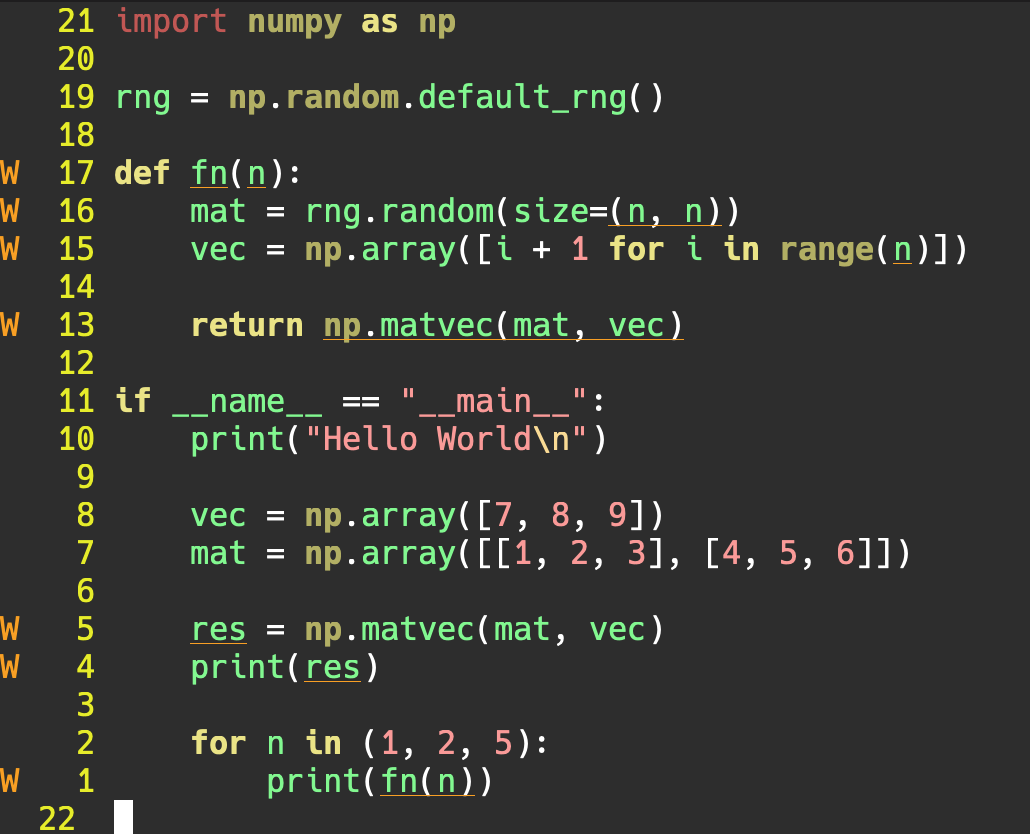
\includegraphics[width=0.5\linewidth]{math3406/using_computers.png}
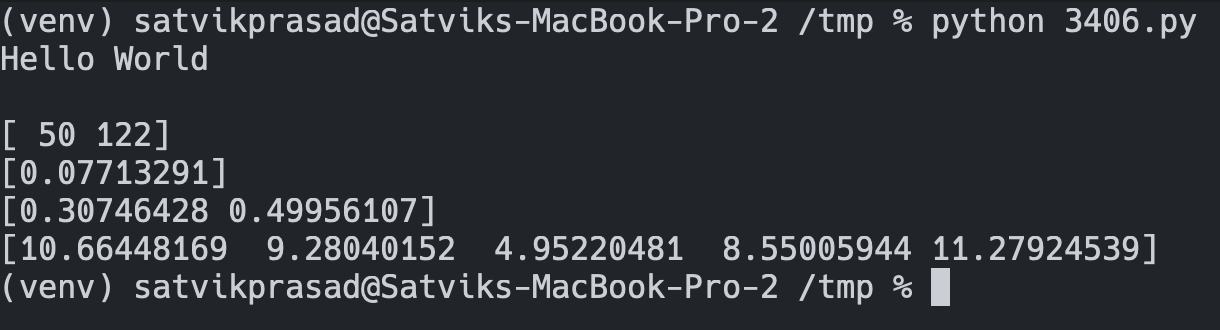
\includegraphics[width=0.5\linewidth]{math3406/Screenshot 2026-08-25 at 8.45.56 am.png}
\end{document}